\documentclass[a4paper,oneside,10pt]{article}

\usepackage[USenglish]{babel} %francais, polish, spanish, ...
\usepackage[T1]{fontenc}
\usepackage[utf8]{inputenc}

\usepackage{lmodern} %Type1-font for non-english texts and characters
\usepackage{graphicx} %%For loading graphic files

\usepackage{amsmath}
\usepackage{amsthm}
\usepackage{amsfonts}
\usepackage{mathtools}

\usepackage{color}
\definecolor{mygray}{rgb}{0.3,0.3,0.3}


\usepackage{listings}

%\lstset{ %
  %basicstyle=\footnotesize,        % the size of the fonts that are used for the code
  %breakatwhitespace=false,         % sets if automatic breaks should only happen at whitespace
  %breaklines=false,                 % sets automatic line breaking
  %captionpos=b,                    % sets the caption-position to bottom
  %deletekeywords={...},            % if you want to delete keywords from the given language
  %escapeinside={\%*}{*)},          % if you want to add LaTeX within your code
  %extendedchars=true,              % lets you use non-ASCII characters; for 8-bits encodings only, does not work with UTF-8
  %keepspaces=true,                 % keeps spaces in text, useful for keeping indentation of code (possibly needs columns=flexible)
  %keywordstyle=\color{mygray},       % keyword style
  %language=C,      			           % the language of the code
  %otherkeywords={*,each,Start,Loop,until,Input,Output},           % if you want to add more keywords to the set
  %numbers=left,                    % where to put the line-numbers; possible values are (none, left, right)
  %numbersep=5pt,                   % how far the line-numbers are from the code
  %numberstyle=\tiny\color{mygray}, % the style that is used for the line-numbers
  %rulecolor=\color{black},         % if not set, the frame-color may be changed on line-breaks within not-black text (e.g. comments (green here))
  %showspaces=false,                % show spaces everywhere adding particular underscores; it overrides 'showstringspaces'
  %showstringspaces=false,          % underline spaces within strings only
  %showtabs=false,                  % show tabs within strings adding particular underscores
  %stepnumber=1,                    % the step between two line-numbers. If it's 1, each line will be numbered
  %stringstyle=\color{mymauve},     % string literal style
  %tabsize=2,	                   % sets default tabsize to 2 spaces
  %title=\lstname                   % show the filename of files included with \lstinputlisting; also try caption instead of title
%}

\lstdefinelanguage{Julia}%
  {morekeywords={abstract,break,case,catch,const,continue,do,else,elseif,%
      end,export,false,for,function,immutable,import,importall,if,in,%
      macro,module,otherwise,quote,return,switch,true,try,type,typealias,%
      using,while},%
   sensitive=true,%
   alsoother={$},%
   morecomment=[l]\#,%
   morecomment=[n]{\#=}{=\#},%
   morestring=[s]{"}{"},%
   morestring=[m]{'}{'},%
}[keywords,comments,strings]%

\lstset{%
    language         = Julia,
    basicstyle       = \ttfamily,
    keywordstyle     = \bfseries\color{blue},
    stringstyle      = \color{magenta},
    commentstyle     = \color{ForestGreen},
    showstringspaces = false,
}

\renewcommand\lstlistingname{Algorithm}% Listing -> Algorithm
\renewcommand\lstlistlistingname{List of \lstlistingname s}% List of Listings -> List of Algorithms


\usepackage{caption}
\DeclareCaptionFormat{myformat}{#1#2#3\hspace{.5mm}\color{mygray}\hrulefill}
\captionsetup[figure]{format=myformat}
\captionsetup[lstlisting]{format=myformat}

\newcommand\note[1]{}
\newcommand\R{\mathbb{R}}
\newcommand\N{\mathbb{N}}
\newcommand\C{\mathbb{C}}
\newcommand\Z{\mathbb{Z}}
\newcommand\Q{\mathbb{Q}}

\newcommand\F{\mathcal{F}}
\DeclareMathOperator*\argmin{arg\,min}
\DeclareMathOperator*\argmax{arg\,max}
\DeclareMathOperator\Var{Var}
\DeclareMathOperator\E{E}
%\DeclareMathOperator\det{det}
\DeclareMathOperator\tang{tang}
\DeclareMathOperator\diag{diag}





\parskip.5\baselineskip
\parindent0mm


\let\oldsection\section
\renewcommand\section{\clearpage\oldsection}


%\usepackage{natbib}
\usepackage{cite}
\usepackage{hyperref}




\begin{document}


\title{Using Numerical Continuation Methods and Galerkin's Method for Finding and Tracing Periodic Solutions in Nonlinear Dynamic Systems} %CITE
\author{Fabian Späh \and Mats Bosshammer}
\date{SS 2016}
\maketitle
\thispagestyle{empty} %No headings for the first pages.


% abstract!

\pagebreak

\thispagestyle{empty} %No headings for the first pages.
\raggedbottom
\tableofcontents %Table of contents
%\cleardoublepage %The first chapter should start on an odd page.

\pagebreak
\pagestyle{plain} %Now display headings: headings / fancy / ...
\flushbottom



\section{Introduction}
% problem statement
% motivation
% general approach
% (outlook on results)

%conventions: lower-scalar, lower,bold-vector, upper,bold-matrix

\section{Modeling Generic Periodic Solutions}



\section{An Optimality Criterion for Periodic Solutions, Galerkin's Method}

%stationary? ordinary?
Given a system of $n \in \N$ real valued, possibly non-linear, stationary, ordinary, coupled, first-order differential equations $\mathbf{x}$
	\begin{equation} \label{eq:SDE}
		\mathbf{x}^\prime = \mathbf{f}(t, \mathbf{x}) \text{, }
	\end{equation}
we are interested in numerically computed, periodic solutions.
That is, solutions $\mathbf{y}: \R \to \R^n$ which obey $\mathbf{y}(t) = \mathbf{y}(t+T)$ for all $t \in \R$ and some period $T \in \R$.
This is the general case, as differential equations of any degree can be converted to a system of degree-$1$ differential equations.

\paragraph{Model} Solution candidates need to be modeled in a certain way.
The periodicity constraint suggests using a multidimensional trigonometric polynomial of degree $m \in \N$
	\[
		\mathbf{y} \coloneqq \sum_{k = -m}^m \mathbf{y}_k \exp\left(i \omega k t\right) \text{,}
	\]
where $\mathbf{y}_k \in \C$, $\mathbf{y}_{-k} = \Re(\mathbf{y}_k) - i \Im(\mathbf{y}_k)$ for $k \in \N$, $-m \le k \le m$, $\omega = \frac{2\pi}T$.
Solution candidates of this form satisfy $\mathbf{y}(t) = \mathbf{y}(t+T)$ by definition.
A function of this form is defined solely by its $m+1$ unique coefficients $\mathbf{y}_k$ for $0 \le k \le m$.

\paragraph{Optimality Criterion} Finding good solutions, that is, functions $\mathbf{y}$ which at least approximate $\mathbf{y}^\prime = \mathbf{f}(t, \mathbf{y})$, requires a measure of fit of the solution.
In this case, Galerkin's method takes this role.
A useful property of the trigonometric polynomial is, that it can be trivially differentiated
	\[
		\mathbf{y}^\prime = \sum_{k = -m}^m i \omega k \mathbf{y}_k \exp\left(i \omega k t\right) \text.
	\]
Employing this property in the definition of the differential equation system yields
	\begin{align*}
			& \mathbf{y}^\prime = \mathbf{f}(t,\mathbf{y})\\
		\Leftrightarrow\ & \mathbf{f}(t,\mathbf{y}) - \mathbf{y}^\prime = 0\\
		\Leftrightarrow\ & \mathbf{f}(t,\mathbf{y}) - \sum_{k = -m}^m i \omega k \mathbf{y}_k \exp\left(i \omega k t\right) = 0 \text.
	\end{align*}

The difference between these two functions is called the \emph{residual} $\mathbf{r}(t) \coloneqq \mathbf{f}(t,\mathbf{y}) - \mathbf{y}^\prime$.
A candidate $\mathbf y$ is a solution iff $\mathbf r = 0$.
%Checking for $\mathbf{r}(t) = 0$ would require comparing the two functions at infinitely many points. %TODO fix... not changed by galerkin
In general the solution of the system of differential equations will not be representable by a trigonometric polynomial.
Galerkin's method relaxes the equality requirement such that only projections on a set of so called \emph{trial vectors}, needs to be zero.
This is equivalent to requiring a projection of $\mathbf{r}(t)$ onto the subspace spanned by the trial vectors to be zero.
Choosing the complex oscillations as a basis for the subspace as well is a solid choice.
Basically the residual is approximated by a trigonometric polynomial and a solution is required to only minimize this representation.
There are other factors supporting this choice: The residual is periodic as well, because of orthogonality many terms can cancel each other out, it allows us to employ the FFT for many operations, and the resulting system of equations is almost balanced.


\paragraph{System of Equations} Because we are only interested in real systems, this yields $m+1$ equations, one for each trial vector $\mathbf{v}_k = \exp\left( i \omega k t \right)$ for $0 \le k \le m$
% = 0
	\begin{align*}
		& \langle \mathbf{r} , \mathbf{v}_k \rangle \\
		=\ & \langle \mathbf{f}(t,\mathbf{y}), \mathbf{v}_k \rangle - \langle \mathbf{y}^\prime, \mathbf{v}_k \rangle \\
		=\ & \langle \mathbf{f}(t,\mathbf{y}), \mathbf{v}_k \rangle - i \omega k \mathbf{y}_k \text.
	\end{align*}
The last step exploits that there is always exactly one component of the candidate function which is not orthogonal to the trial vectors.
However, there are $m+2$ variables: $m+1$ unique coefficients and $\omega$.
This represents the situation, that at this point there is still one degree of freedom: Each phase shifted version of a solution is still a solution.
We thus introduce another generic equation called the \emph{anchor} equation, which basically chooses one of these solutions.
In this case $\langle \mathbf{y}(0), (\delta_{1i})_{i \in \N_n} \rangle = 0$ is used:
For $t = 0$, the solution needs to intersect the hyperplane defined by being zero in the first component.
This can be formulated by requiring the corresponding coefficients to sum up to zero.
The anchor equation needs to be adapted to the system considered: If there are no intersections with this plane, another equation needs to be chosen.

%motivation tedious, error prone
When transferring these theoretical constructs to a practical setting, the main change is that solutions $\mathbf{y}$ are not considered to be functions of continuous time, but vectors representing discrete time.
Let $N = 2m+1$, then
	\[
		\mathbf{\mathbf{y}} = \left( \sum_{k=0}^{N-1} \mathbf{y}_k \exp\left(i \frac{2\pi}{N} j k\right) \right)_{0 \le j \le N-1} \text.
	\]
This is no real limitation at that point, as solution candidates are band limited by construction.
Define the \emph{DFT matrix} $\mathbf F \in \R^{N \times N}$ and the coefficient vector $\mathbf Y \in \left(\C^n\right)^N$
	\begin{align*}
		\mathbf{F} &\coloneqq N^{-1} \left( \exp\left(-i \frac{2\pi}{N} j k \right) \right)_{0 \le j,k \le N-1} \\
		\mathbf{Y} &\coloneqq \left(\mathbf{y}_k\right)_{0 \le k \le N-1} \text.
	\end{align*}
$\mathbf Y$ is a vector of vectors, while somewhat unusual, allows for more concise notation than notation as a matrix.
Using these constructs allows us to reformulate
	\[
			\mathbf{y} = \mathbf{F^{-1}} \mathbf{Y} \text.
	\]
Considering only the equations from projection onto a trial vector and considering $\omega$ to be known, and let $\mathbf K \in \R^{N \times N}$ be the diagonal matrix with entries going from $0$ to $m$ to $-m$, the system of equations becomes %TODO define
	\[
		\mathbf{F} \mathbf{\tilde f}(\mathbf F^{-1} \mathbf{Y}) - i \omega \mathbf K \mathbf Y = 0\text,
	\]
where $\mathbf{\tilde f}: (\R^n)^N \mapsto (\R^n)^N$ simply row wise applies $\mathbf{f}$, the function defining the system of differential equations, see \autoref{eq:SDE}.

Introducing these new constructs might at first glance appear unnecessarily complicated, because the system of equations was already known, and could be used in the state it was in.
However, an implementation in the basic form would have required different treatment for each dynamic system, while this reworked form is only trivially dependent of the system and the degree of the trigonometric polynomial.
That is, the auxiliary vectors and matrices are trivially constructed, as is $\mathbf{\tilde f}$ from $\mathbf f$.
While knowing the system of equations is important, the core task of finding a good solution requires the Jacobian of the system.
The by far largest advantage is that from this form, the system can be derived in a general way.

Let $D$ denote a differential operator.
The only variable in the system is $\mathbf Y$, thus
	\begin{align}
			& D \left( \mathbf{F} \mathbf{\tilde f}(\mathbf{F}^{-1} \mathbf{Y}) - i \omega \mathbf K \mathbf Y \right) \nonumber \\
		%=\ & \mathbf{F} \frac{d}{d\mathbf Y}\mathbf{\tilde f}(\mathbf{F}^{-1} \mathbf{Y}) - i \omega \mathbf K \\ 
		=\ & \left(\mathbf{F} \mathbf J_{\mathbf{\tilde f}} \left( \mathbf{F}^{-1} \mathbf{Y} \right) \mathbf{F}^{-1} - i \omega \mathbf K \right) \cdot D \mathbf Y \label{eq:vecsys}\text,
	\end{align}
	
	%TODO careful: dY/dY != I

where $\mathbf J_{\mathbf{\tilde f}} \coloneqq \frac{d \mathbf{\tilde f}(\mathbf Y)}{d\mathbf Y}$ is the Jacobian of $\mathbf{\tilde f}$, a vector-by-vector derivative, which yields a matrix.
However, because both vector's elements are vectors themselves, the entries of the matrix are again vector-by-vector derivatives.
This results in an $N \times N$ matrix of matrices with
	\[
			\left(\mathbf J_{\mathbf{\tilde f}}\right)_i^j = \frac{d}{d\mathbf x_j} \mathbf f (\mathbf x_i) = \delta_{ij} \mathbf J_\mathbf f(\mathbf x_i) \text, %TODO fix x
	\]
where $\mathbf J _ \mathbf f \coloneqq \frac{d \mathbf f(\mathbf x)}{d\mathbf x}$ is the Jacobian of $\mathbf f$.
The matrix $\mathbf J_{\mathbf{\tilde f}}$ is diagonal, thus
	\[
		\mathbf J _ \mathbf{\tilde f} (\mathbf Y) = \diag\left( \left(\mathbf J _ \mathbf f \left(\mathbf Y_i\right) \right)_{i \in \N_N} \right)
	\]
Because different cells of $\mathbf J_{\mathbf f}$ are independent, the expression for the Jacobian of the whole system can be considered separately for each partial derivative in $\mathbf J _\mathbf f$.
For $k,l \in \N_n$ define the $N \times N$ diagonal matrix which extracts a single partial derivative
	\[
		\mathbf A_{kl}(\mathbf Y) = \diag\left( \left(\frac{\partial f_k}{\partial x_l} \left(\mathbf Y_i\right)\right)_{i \in \N_N} \right) \text.
	\]
For each $k$ and $l$ \autoref{eq:vecsys} then becomes
	\begin{equation}
		\left( \mathbf{F} \mathbf A_{kl}(\mathbf{F}^{-1} \mathbf{Y}) \mathbf{F}^{-1} - i \omega \mathbf K \right) \cdot D \mathbf Y
	\label{eq:syssingle}
	\end{equation}
This expression is again free of nested vectors.

%Because of the diagonal structure of the matrix, the term $\frac{d\mathbf{\tilde f}}{d\mathbf x}(\mathbf{F}^{-1} \mathbf{Y}) \mathbf{F}^{-1}$ is essentially a multiplication of each row of $\mathbf F^{-1}$ with a constant.
Because $\mathbf A_{kl}(\mathbf{F}^{-1} \mathbf{Y})$ is diagonal, $\mathbf A_{kl}(\mathbf{F}^{-1} \mathbf{Y}) \mathbf{F}^{-1}$ is the rows of $\mathbf F^{-1}$ each multiplied by a constant.
This can also be seen as an element wise multiplication of the columns of $\mathbf F^{-1}$ by a column vector defined by the diagonal of $\mathbf A_{kl}(\mathbf{F}^{-1} \mathbf{Y})$:
	\begin{align*}
		&\mathbf c_k \coloneqq \left(\exp\left(i\frac{2\pi}{N} j k\right)\right)_{0 \le j \le N-1}\\
		&\mathbf d \coloneqq \frac{\partial f_k}{\partial x_l} \{\mathbf Y\} \text.
	\end{align*}	
A column of $\mathbf{F} \mathbf J_{\mathbf{\tilde f}} \left( \mathbf{F}^{-1} \mathbf{Y} \right) \mathbf{F}^{-1}$ is then the transform of the product of two signals $\mathcal F(\mathbf d \cdot \mathbf c_k)$.
Because of the structure of $\mathbf c_k$, this corresponds to a simple periodic shift of the Fourier coefficients of the discrete signal $\mathbf d$ by $k$ steps.
Using this for every column of the complete term yields
	\[
			\mathbf{F} \mathbf A_{kl}(\mathbf{F}^{-1} \mathbf{Y}) \mathbf{F}^{-1} = \left( \mathbf \F(\mathbf d)_{((i-j))_N} \right)_{0 \le i,j \le N} \text,
	\]
that is, a simple circulant matrix.



\section{Finding Periodic Solutions}
\label{sec:initial}

A separate problem from evaluating, optimizing and continuing periodic solutions is finding an initial candidate solution.
Because continuation is a crucial part of this project, having just one single periodic solution might enable to find many others, through tracing and switching solution branches.
Because the systems considered in this work have stable periodic solutions, we focus on this case.
When this is not the case, as mentioned in the section about continuation methods (\autoref{sec:cont}), a homotopy between a trivial system and the target system, combined with continuation methods, might be a promising approach.

Starting from a point in the periodic solution's basin of attraction, one can simply forward integrate such a system.
There are several possible problems involved:
\begin{itemize}
	\item Forward integration can accumulate errors.
	\item Even if the starting point lies exactly on the periodic trajectory, the sampling interval would probably not be an integer fraction of the period of the periodic trajectory.
		Periodicity in the sequence of points are not directly related to periodicity in the continuous system.
	\item Given the nature of the project, it is very likely that period doubling bifurcations are encountered.
		These provoke situations where two periodic solutions exist which are difficult to distinguish.
\end{itemize}

Forward integration yields a sequence of points in phase space $(\textbf{s}_i)_{i \in \N}$.
To obtain more manageable data only intersections of the trajectory with a hyperplane $p(\textbf{x}) = \langle \textbf{n}, \textbf{x}-\textbf{x}_0 \rangle = 0$ in a single direction are considered (so called Poincaré sections).
To find these, $\textbf{s}_i, \textbf{s}_{i+1} = \textbf{s}_i + h_0 \cdot \textbf{f}(\textbf{s}_i)$ with $p(s_i) \le 0 < p(s_{i+1})$ are searched.
Because of continuity, there needs to exists $h \in [0,h_0]$ such that $p(\textbf{s}_i + h \cdot \textbf{f}(\textbf{s}_i)) = 0$, which is found via bisection.
Let $(\textbf{u}_i)_{i \in \N}$ be the sequence of intersections.

To find the number of intersections per period, the intersections are partitioned into $k \in \N$ disjoint clusters $V_{k,i} = \{ \textbf{u}_m\ |\ m \in k\N+i \}$ for $i \in \N$, $i \le k$.
The relative quality of the $i$-th cluster can then be assessed using the within-cluster variance $\sum_{v \in V_{k,i} } ||v - \E(V_{k,i})||^2$.
The correct number $k_{\text{min}} \in \N$ of intersections in one period is then taken to be the one minimizing the sum of within-cluster variances:
\[
	k_\text{min} \coloneqq \argmin_{k \in \N} \sum_{i = 1}^k \sum_{v \in V_{k,i} } ||v - \E(V_{k,i})||^2 \text.
\]
For further information about these measures see for example \cite{halkidi2001clustering}. %TODO measure...

In this form the criterion might at best work if the intersection sequence is infinite.
When dealing with finite sequences increasing the number of clusters inevitably leads to lower total within-cluster variances.
It is thus necessary to constrain the available values for $k$ and discourage the method of overestimating the number of clusters.
Trivially an upper limit for $k$ needs to be introduced.
Furthermore, the minimality criterion needs to be relaxed: Suppose there are $k_\text{min}$ intersections per period, then all multiples of $k_\text{min}$ yield equal or lower ratings.
One thus wants to choose the minimum $k$ which is in some sense still almost optimal.


\section{Tracing Periodic Solutions, Predictor-Corrector Continuation}
\label{sec:cont}

A central part of this project are numerical continuation methods.
Being a large topic, the details are out of the scope of this work, we thus concentrate on conveying a general idea of the concepts.
This is especially true for the wealth of methods from other fields, numerical continuation draws upon.
Among the things required in the following are basic knowledge of Newton's method in multiple dimensions, forward integrating differential equations (Runge-Kutta methods) and basic vector calculus (Jacobian matrix).
For a more thorough introduction to the topic, please refer to~\cite{allgower1990numerical}, on which the continuation part of project and this section of this document is based.

The base of numerical continuation is formed by the fact that in the vicinity of a solution of an underdetermined continuous system, there are almost always other, similar solutions.
Iterative application of this, in the context of systems having one constraint less than unknowns, yields that solutions of the system form a curve (which might be closed).
Continuation methods provide means to trace these curves, and thus to derive infinitely many other solutions from a single given solution.
A very central use-case of such a method is being able to numerically solve a system without requiring an otherwise needed good starting value.
This works by continuously blending two systems with equal numbers of unknowns and equations using a homotopy, which adds one degree of freedom.
This way, a known solution from a system can be traced to one of the harder system.
However, in the context of this work, where the underdetermination occurs naturally, we are not interested in single solutions but rather in obtaining the whole continua of solutions.

This project uses a single continuation method: The predictor-corrector method.
As the name suggests, it continues the solution curves, by predicting the next point on the curve through linearization at the current point, and afterwards correct it, to compensate for the non-linear influences.


%implicit function theorem

\section{Case Study: Lorenz System}

The Lorenz system is defined by
\begin{align*}
	\dot x &= \sigma (y-x)\\
	\dot y &= x(\rho-z)-y\\
	\dot z &= xy-\beta z \text,
\end{align*}
where $\sigma = \beta = 0.1$ and $\rho$ is the variable parameter.

As a reduction operator for the creation of the bifurcation diagram
\[
	\mathbf y \mapsto \{||\mathbf y(t) - \mathbf a||\ |\ t \in [0,2\pi),\ \mathbf y_3(t) = \rho + 7\}
\]
is used, where $\mathbf a = (\sqrt{\beta(\rho-1)}, \sqrt{\beta(\rho-1)}, \rho-1)^T$ is one of the fixed points of the system.
It maps a solution to the distances of its intersections with the $z = \rho+7$ plane to the fixed point $\mathbf a$.
This particular choice was made empirically, as most other choices result in changing numbers of intersections for single solution branches, too many intersections or result in many lines overlapping one another.

The system features stable periodic solutions for $\rho \in \{99.65, 100.5, 160, 350\}$.
These values are used as starting points for the creation of the bifurcation diagram.
The general process of finding a stable solution, tracing it to a bifurcation point or until otherwise satisfied, doubling the period and finding period doubling bifurcations is the same as for the Rössler system.

See figures \ref{fig:lorenzfull}, \ref{fig:lorenzcut} for visual results.
The tracing of the solutions for $\rho \to 0$ had to be suspended, because it became too slow to be practical.
See the discussion in \autoref{sec:outro} for details.

\newgeometry{top=0cm}

\begin{figure}
\centering\makebox[0pt]{\rotatebox{90}{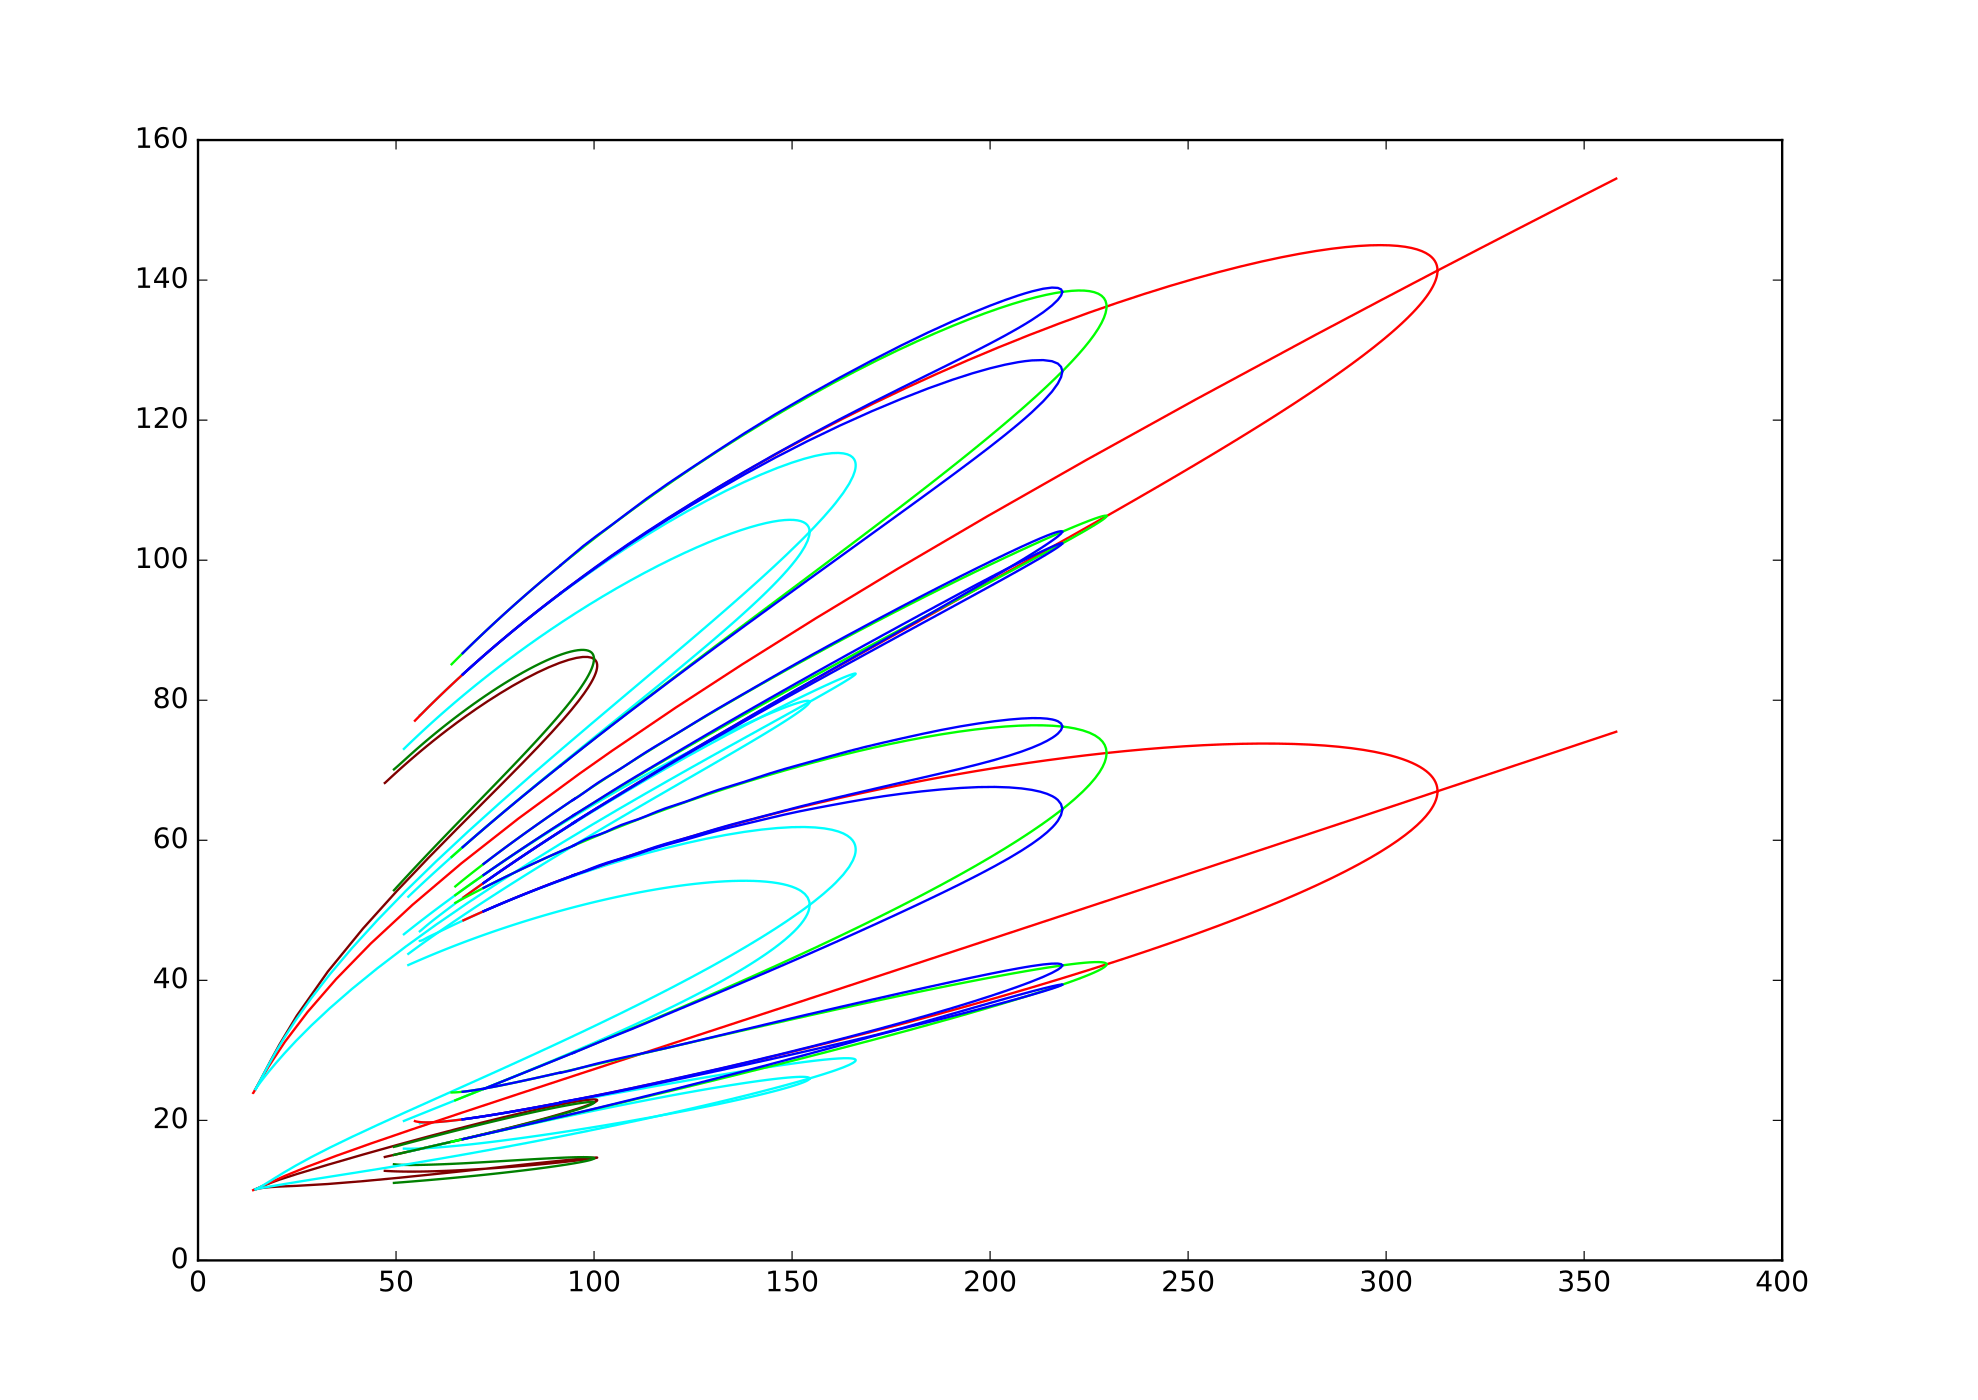
\includegraphics{img/lorenzoverview.png}}}
\caption{
	An overview of the Lorenz bifurcation diagram.
}
\label{fig:lorenzfull}
\end{figure}


\begin{figure}
\centering\makebox[0pt]{\rotatebox{90}{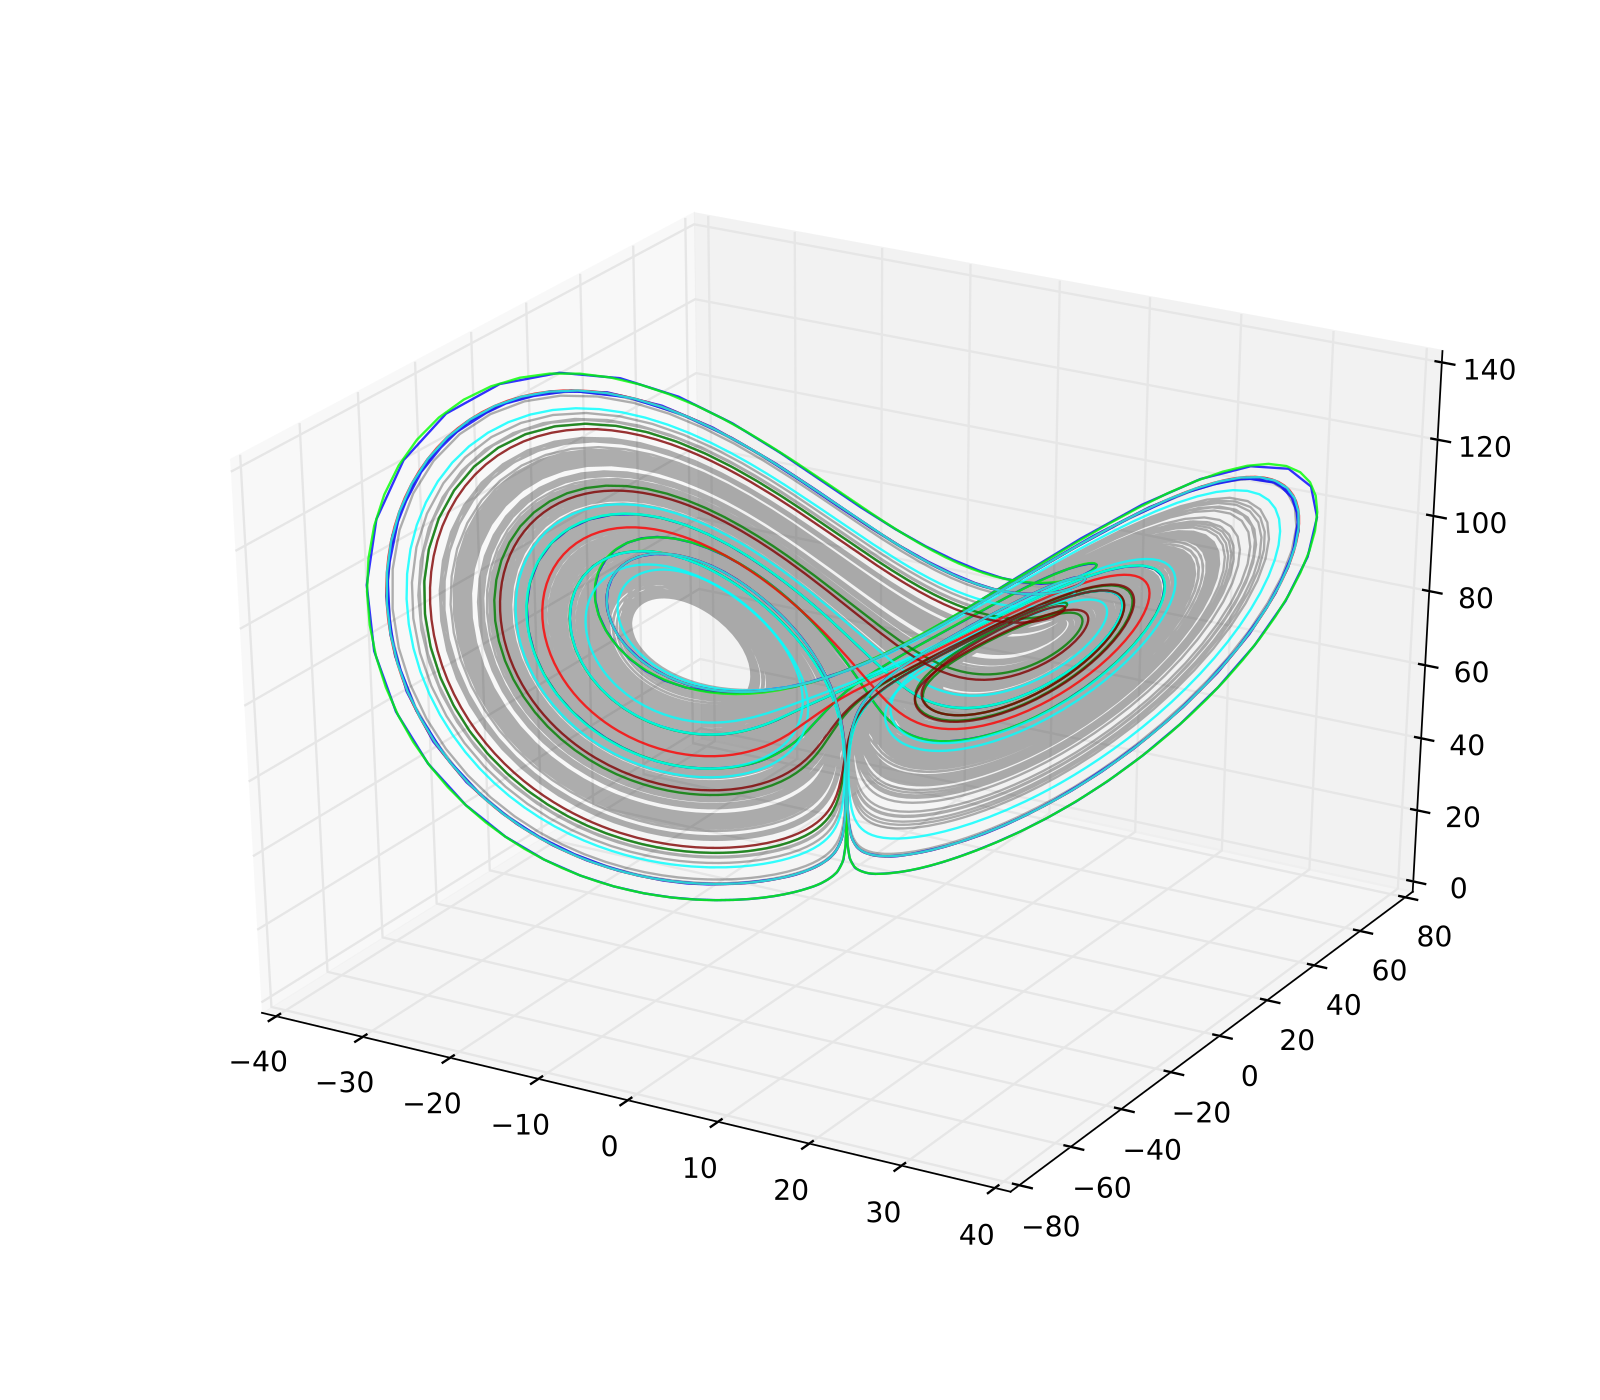
\includegraphics{img/lorenzcut80.png}}}
\caption{
	The periodic orbits for $\rho=80$, together with an underlying trajectory obained through forward intergration (grey) in phase-space. 
	The colors of the periodic solutions match the bifurcation diagram.
}
\label{fig:lorenzcut}
\end{figure}

\restoregeometry

\section{Case Study: Rössler System}

The well known Rössler system is given by the equations
\[
	\begin{array}{rcl}
		\dot x &=& -y - z \\
		\dot y &=& x + a \cdot y \\
		\dot z &=& b + z \cdot (x - c) \\
	\end{array}
\]
with parameters $a$, $b$, and $c$. For this example, $a$ and $b$
are fixed to $0.1$, while we are varying $c$.

The system has several periodic solutions for each value of $c$ with different
periodicities, though only one is stable at a time. We are interested in the origin and
branching of those solutions and, thus, drawing a bifurcation diagram using the map
\[
	f \mapsto \{ \|f(t)\|_2  \ | \ t \in [0, 2\pi), \ f(t)_1 = 0 \} \ .
\]
Here, $f$ denotes a single periodic solution. Note, that we use only the approximation
given by Galerkin's method.

Now, the exploration of the bifurcation with the given tools follows rougly this steps:
\begin{enumerate}
	\item As a starting point, search for a value of $c$ such that the system has a
		stable, periodic solution and use the method described in
		\autoref{sec:initial} to find it. 4000 iterations in the transient part with step
		size of $0.01$, 120 generated intersections with the $(x=0)$-plane and tests for
		at most $30$ periods were sufficient for all initial solutions of the Rössler
		system. We started at $c=4$ with $64$ samples.
	\item Trace out the branch just by following the newly found solution in both directions
		using the predictor-corrector continuation method (\autoref{sec:cont}). The
		parameters $\kappa=0.4$, $\delta=3.0$, and $\alpha=10.0$ are a decent choice for
		the whole diagram as a good tradeoff between performance and accuracy.
	\item It is possible to detect a pitchfork bifurcation by doubling up the periodicity
		artifically. Using the described predictor-corrector method, the value
		of $c$ will eventually converge to the bifurcation point, i.e., a point with a
		singular tangent. Since the method is now stuck, reaching the doubly-periodic
		solution can be done by solving a slightly perturbed problem for a short time.
		A short perturbation of strength $0.2$ was enough to reach the doubly-periodic
		solution. Also, it might be necessary to increase the sample size due to increased
		complexity in the descending branch.
	\item Remove the perturbation and continue tracing out the bifurcation, i.e. start
		over in 1 or 2.
\end{enumerate}

\begin{figure}[!ht]
	\centering
	\subfloat[][]{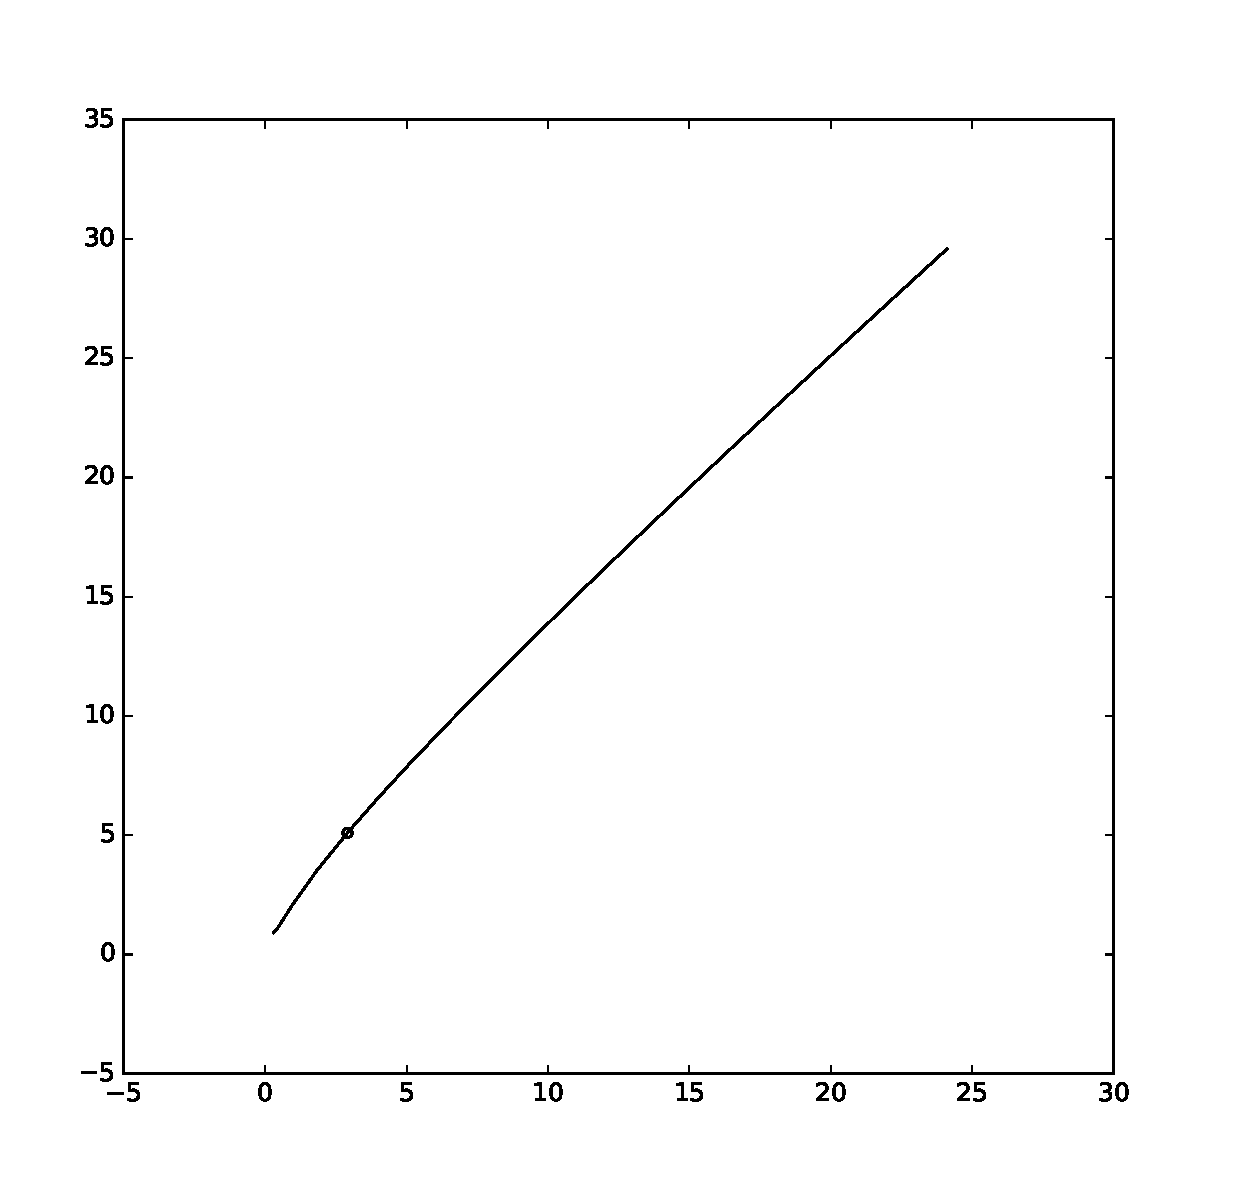
\includegraphics[width=.4\textwidth]{img/roessler1a.pdf}}\quad
	\subfloat[][]{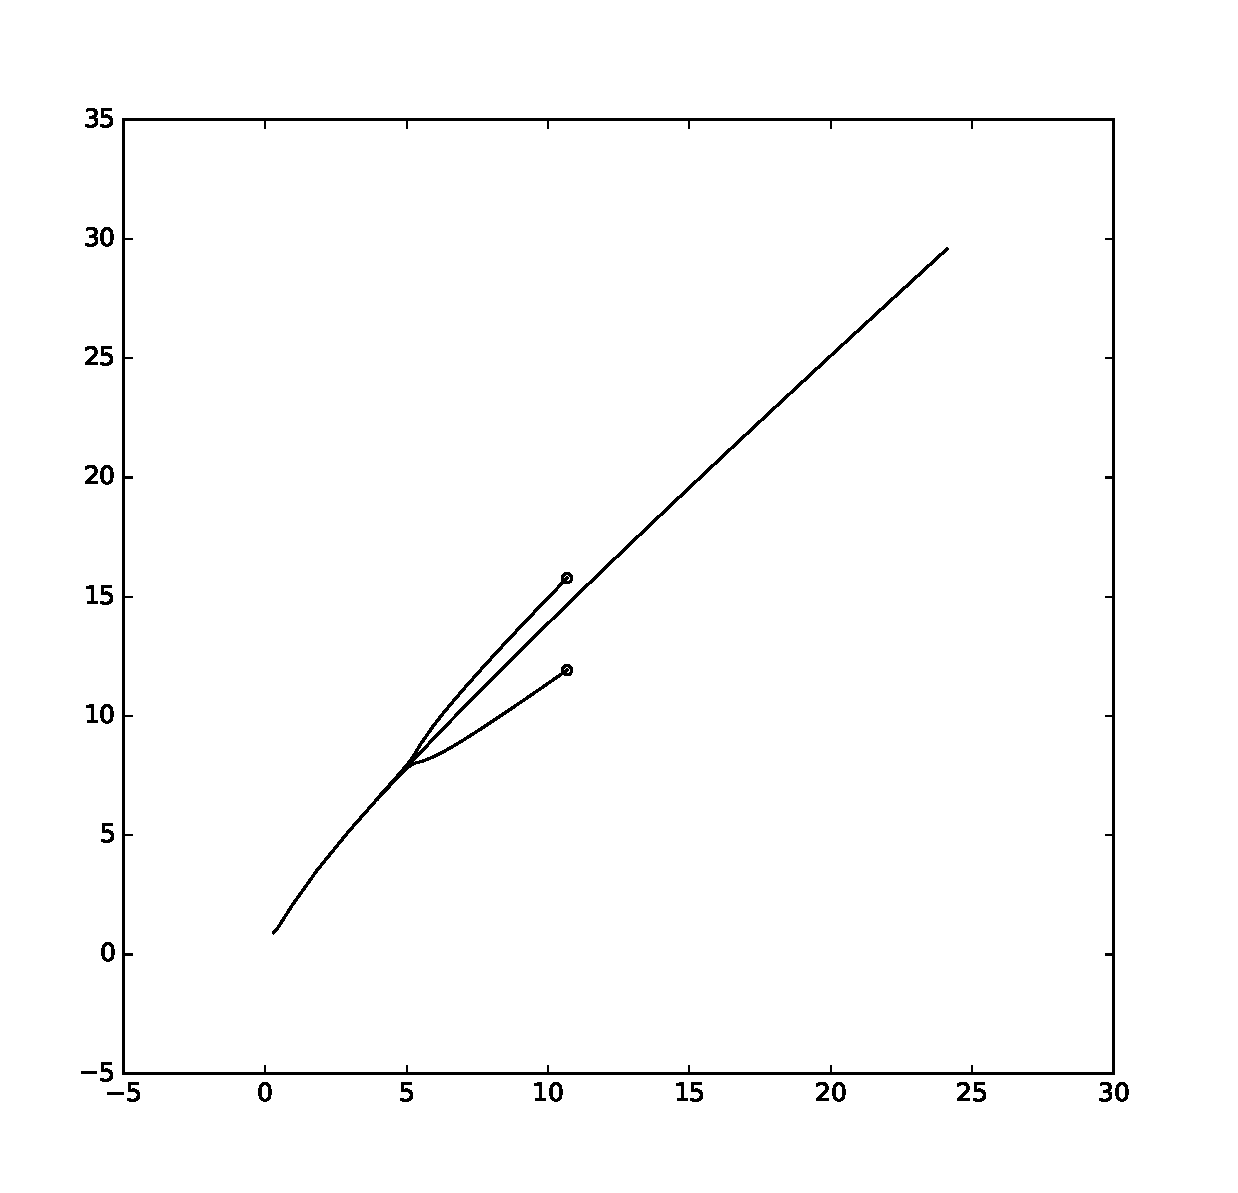
\includegraphics[width=.4\textwidth]{img/roessler1b.pdf}}\\
	\subfloat[][]{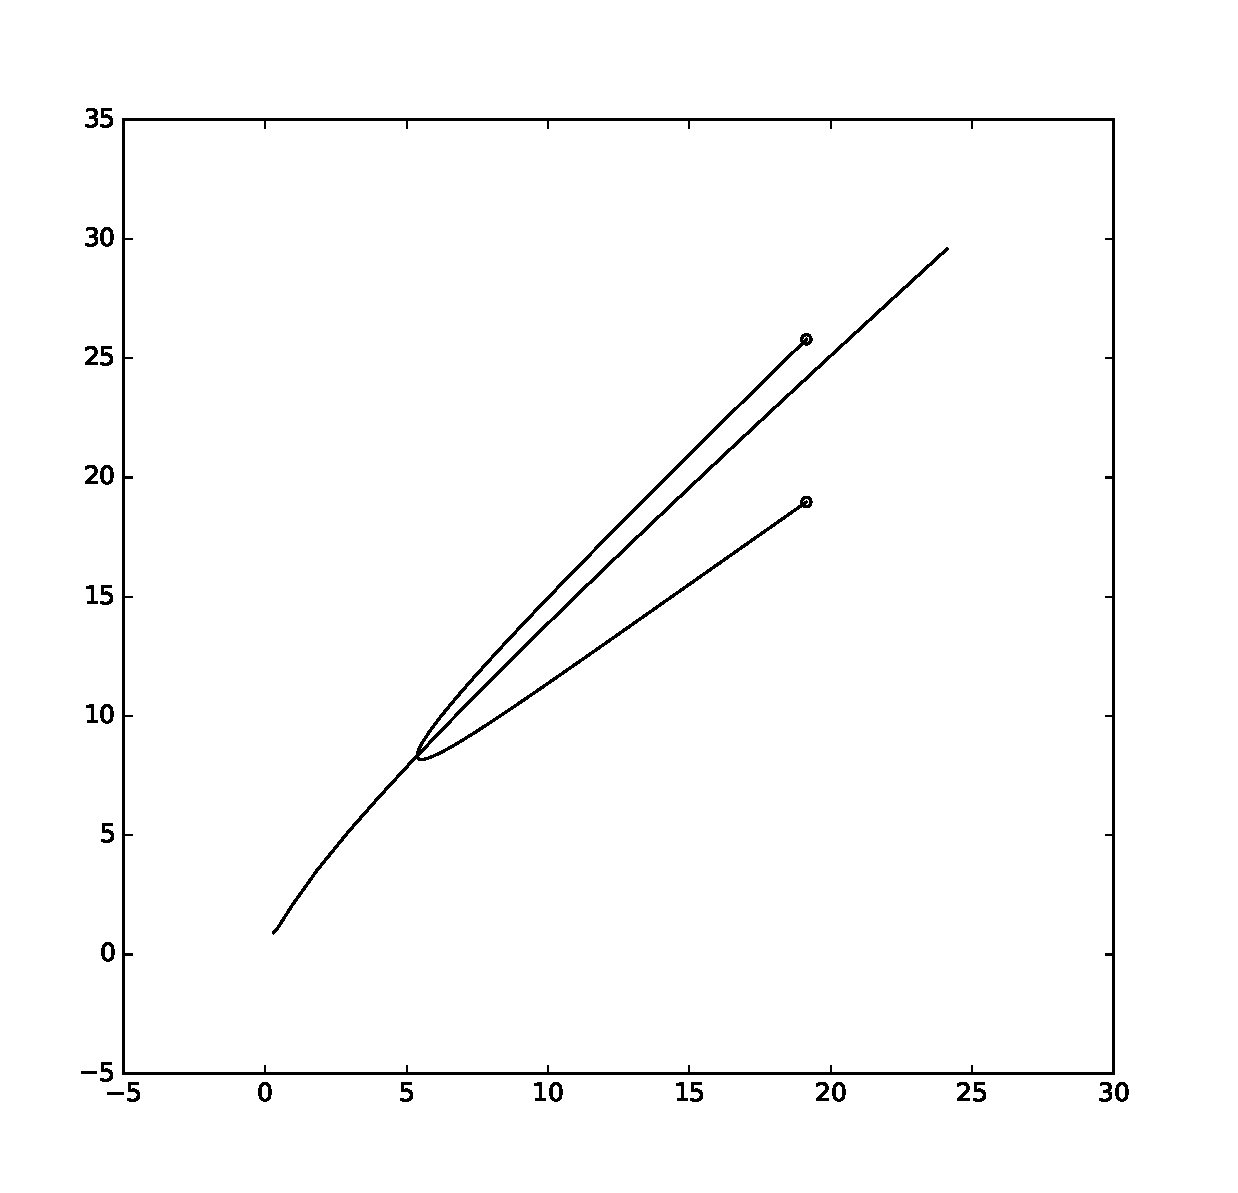
\includegraphics[width=.4\textwidth]{img/roessler1c.pdf}}\quad
	\subfloat[][]{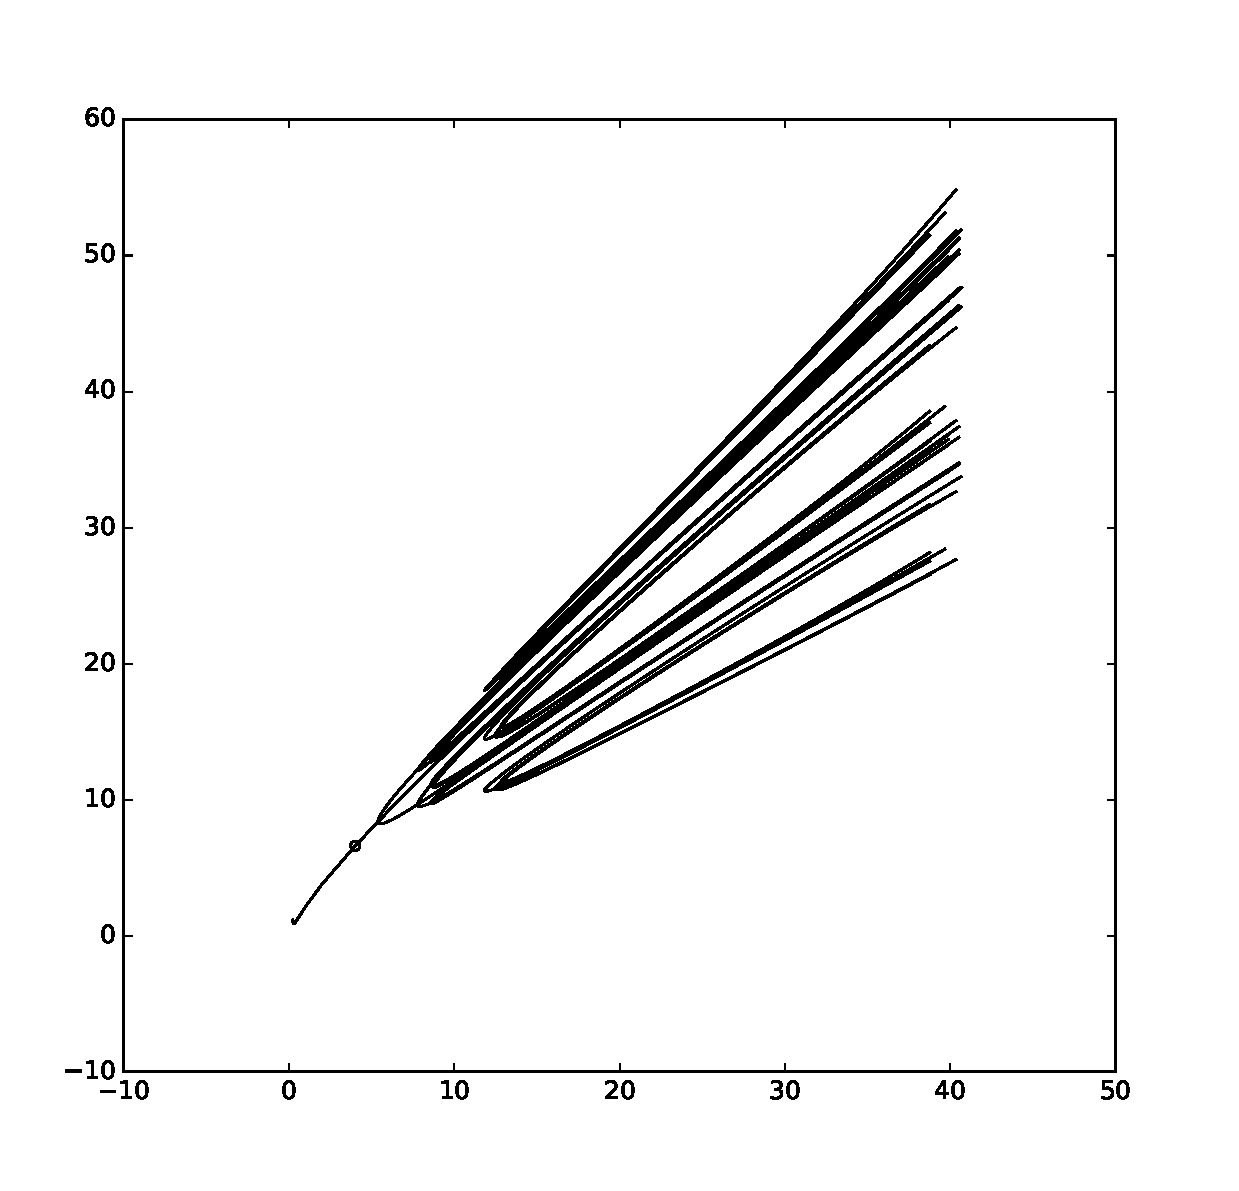
\includegraphics[width=.4\textwidth]{img/roessler1d.pdf}}
	\caption{Tracing out the branch of solutions beginning with the solution for
	$c=4$ (a). The bifurcation point in $c \approx 5.376$ is avoided by using a permutation (b),
	and the two-periodic solutions can be traced out after removing the inaccurate values
	from before (c). Eventually, we reach (d), a widely traced out bifurcation diagram.
	Note the solutions with periodicity three and descendants, that do not originate in
	the peridocity-one branch.}
\end{figure}

\begin{figure}[!ht]
	\centering
	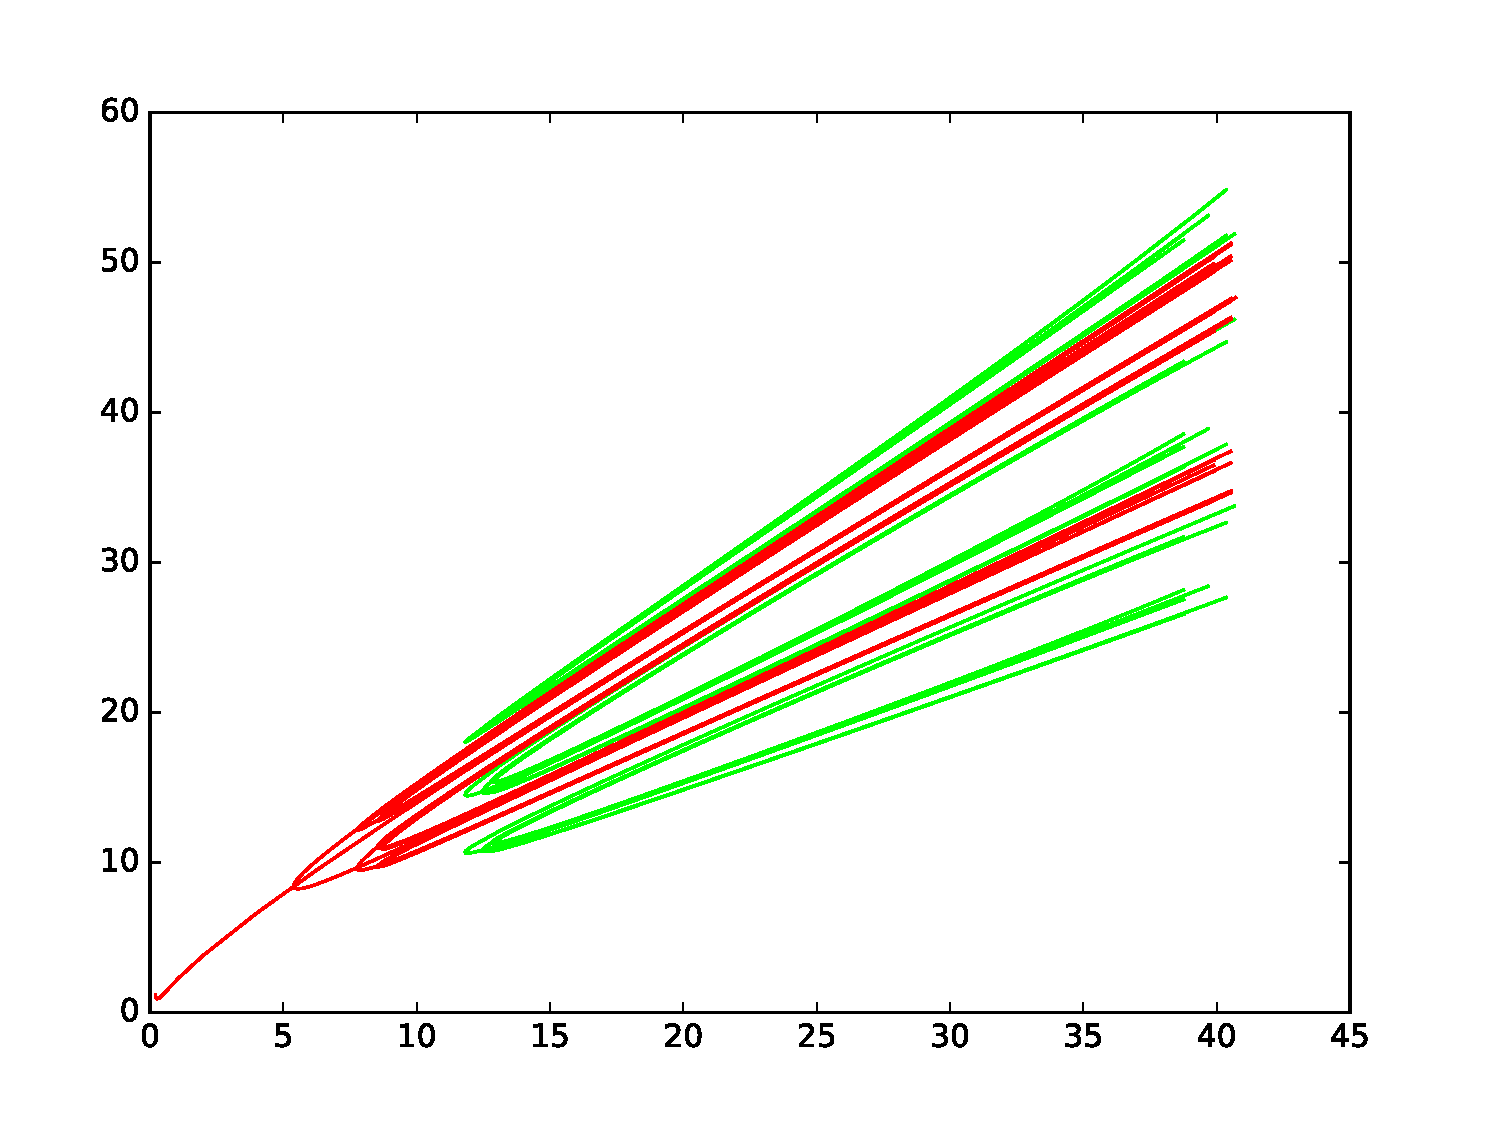
\includegraphics[width=1\textwidth]{img/roessler2a.pdf}
	\caption{The bifurcation diagram of the Rössler system for varying $c$. The
		even-periodic solutions are colored red, the odd-periodic ones green.}
\end{figure}

\begin{figure}[!ht]
	\centering
	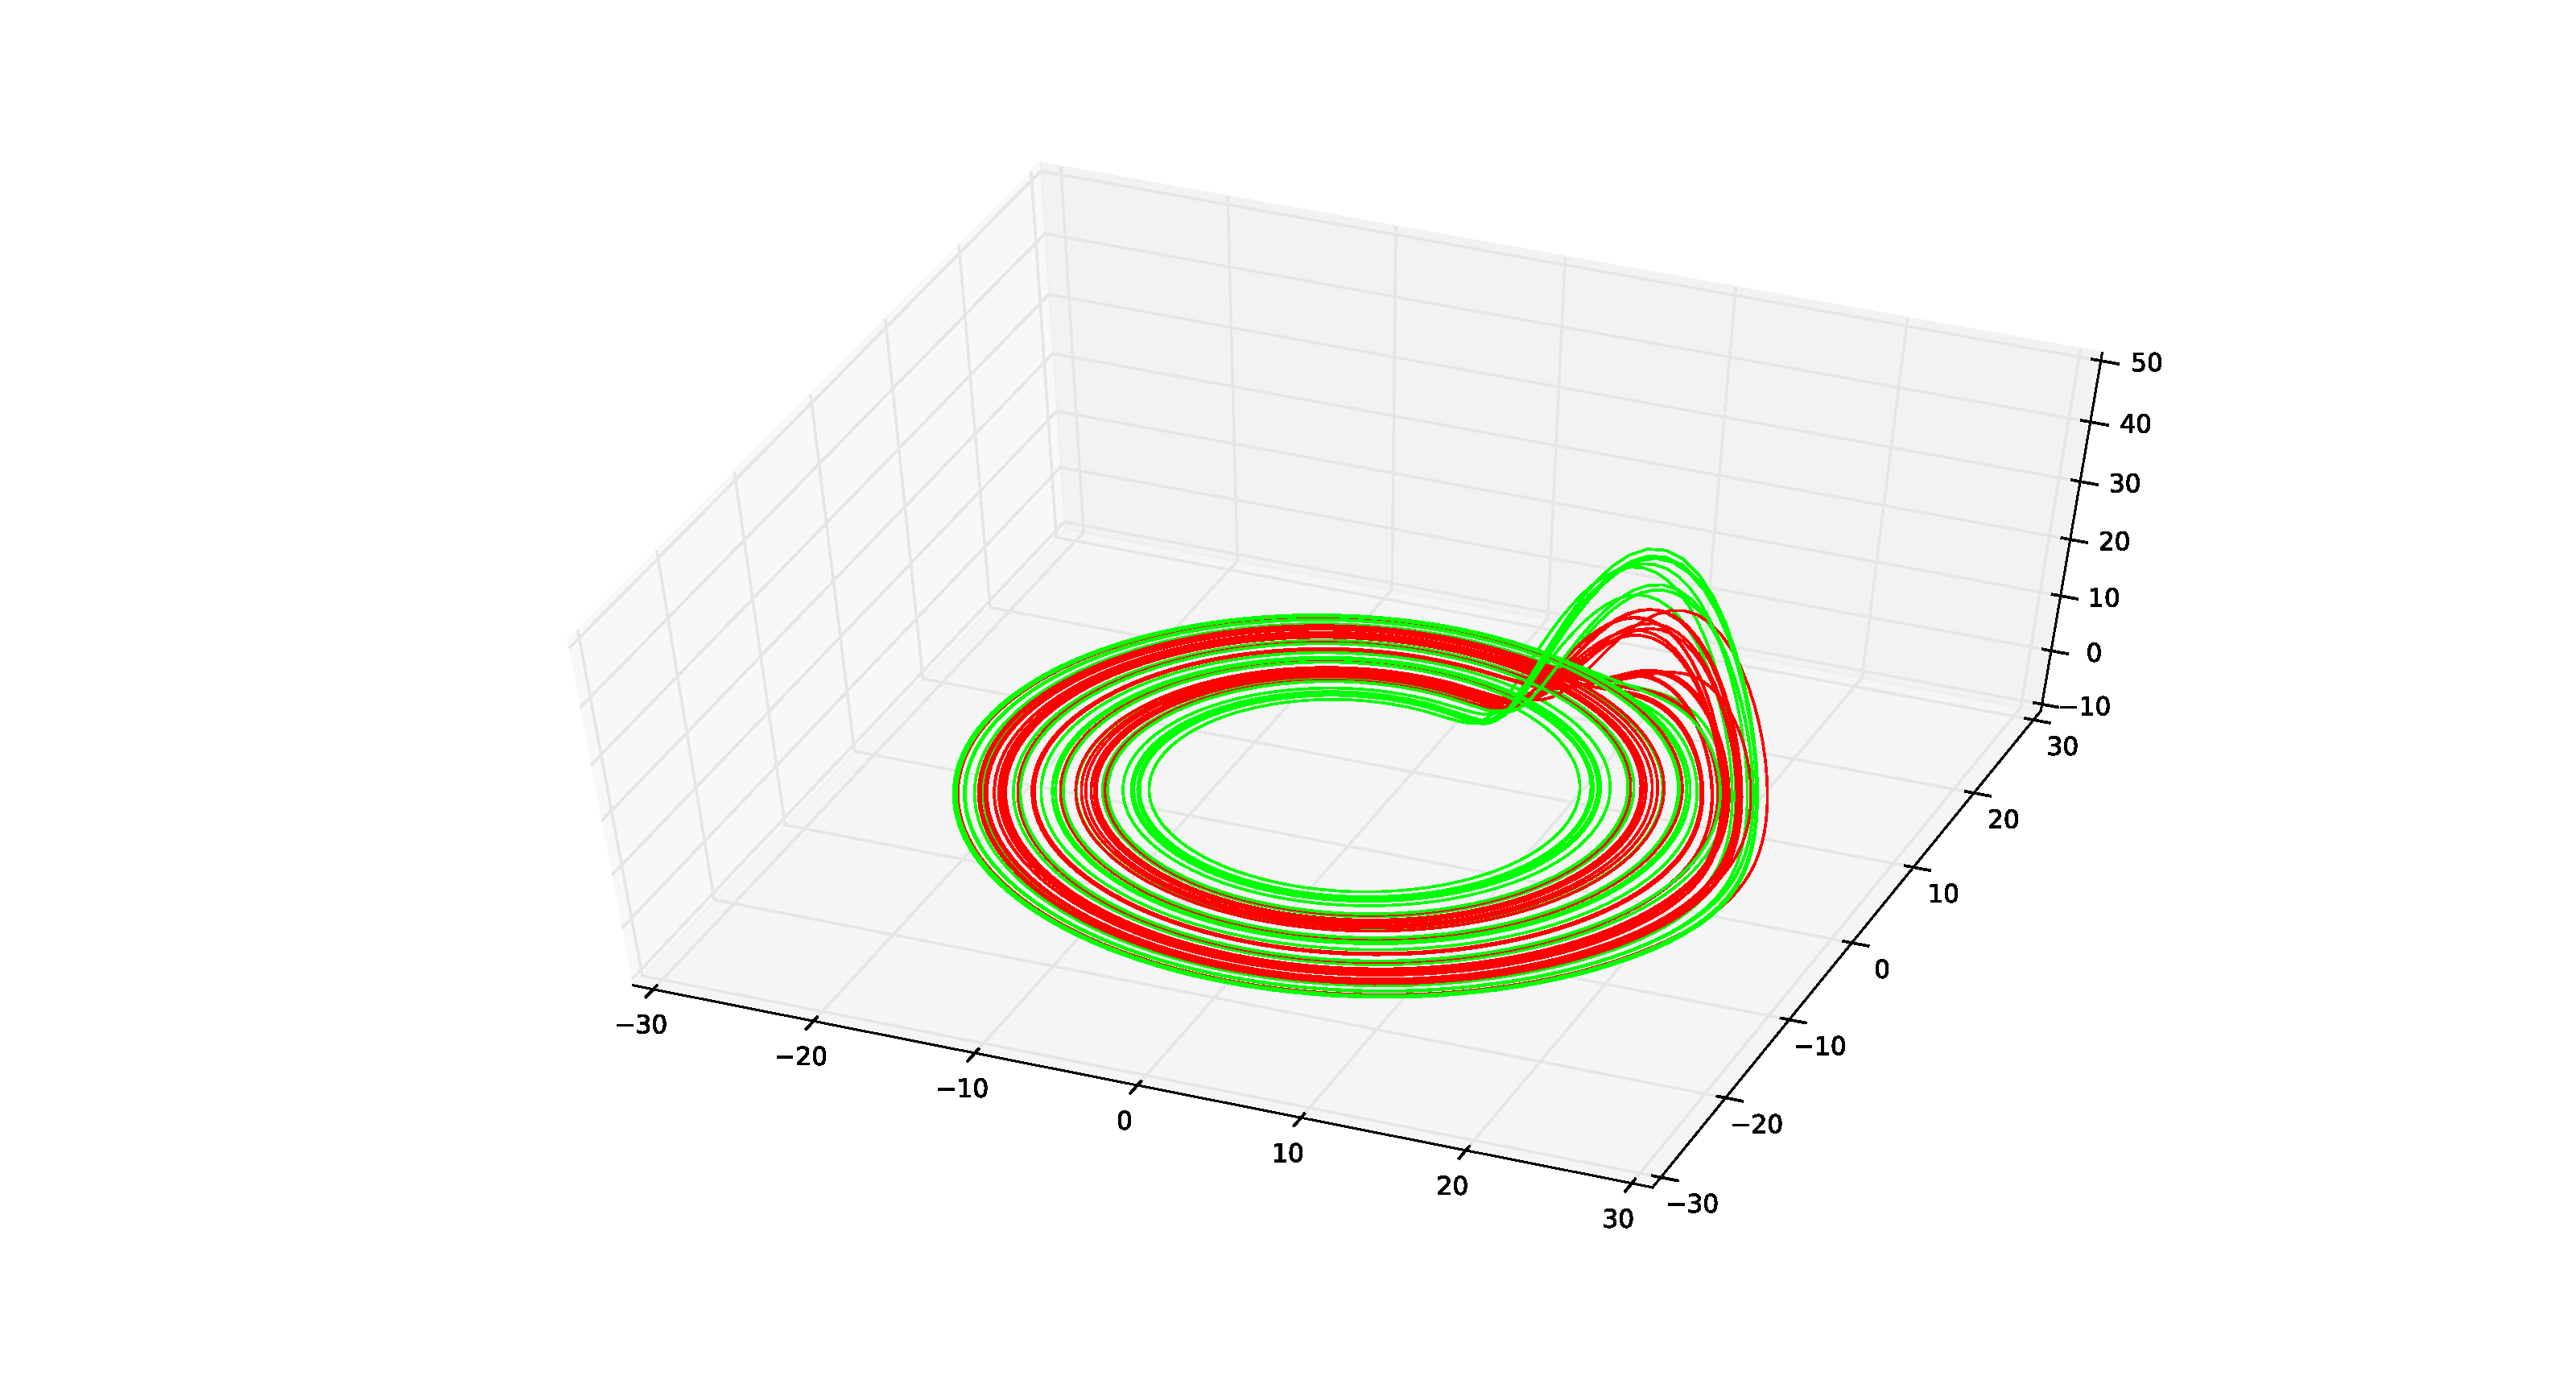
\includegraphics[width=1\textwidth]{img/roessler2b.pdf}
	\caption{All found solutions for $c=\dots$ plotted into one diagram.
	Observe how the odd-periodic and even-periodic solutions dodge since they do not
	originate from each other.}
\end{figure}





\section{Results \& Outlook}

The project's goals of interactively creating bifurcation diagrams using Galerkin's method and continuation methods could be met.
There are some further points of interest.
On a practical level, one of the things an implementation of the sort of this project might benefit from are Broyden updates.
In its basic form, the method allows to update the Jacobian of the system of equations obtained from the Galerkin operator.
Though calculating the Jacobian is a time-consuming task, this is of minor interest, as the effort is negligible compared to the effort for inverting the Jacobian, which is needed for each computation of the tangent.

One of the main sources of complications are orbits which change their direction too fast.
As is the case in the Rössler system for high values of $\gamma$ and in the Lorenz System for low values of $\rho$. %pics
In these regions the optimization procedure converges slowly and the predictor-corrector method's step-size adaption suggests very small steps (as seen from the bifurcation view).
There is a variety of possible reasons
\begin{description}
	\item[Numerical] Certain values, for example in the Jacobian, are not representable sufficiently precise.
	\item[Modeling] A trigonometric polynomial of finite degree can not be used to model infinitely sharp turns.
		The numerical cause is likely to be a consequence of this choice for a model.
\end{description}
No attempts were made to investigate the definite cause of this behavior, however, choosing a model which is more adapted to these challenges might allow for more accurate results in these areas.
Furthermore, solution branches could be traced further, as these effects are a cause of stopping the tracing of solutions in the Rössler, as well as in the Lorenz system. %ref
While in the case of the Rössler system this is less of a problem, as the solutions for high $\gamma$ did not appear to reveal anything of immediate interest, in the Lorenz system the behavior prohibited tracing the solutions in the $\rho \in (0,2)$ area.
It is this area, where there is a huge amount of interaction between the branches of solutions.

Modeling the trajectories as linear combinations of non-equidistant B-splines instead of complex oscillations might yield interesting results. %cite
\begin{itemize}
	\item The periodicity requirement can be enforced by choosing the basis vectors appropriately.
	\item Through adaption of the knots, the degree of smoothness can be varied to the point being $C^0$ only.
		This can be done by changing \emph{multiplicities} of knots, that is, by having several knots be equal.
		An interesting point is that this change in continuity can occur dynamically through optimizing the knot vector.
\end{itemize}



\bibliography{bibliography}{}
\bibliographystyle{apalike}




\end{document}
